\documentclass{jors}

%% Set the header information

% Commenting out as this overrides the section titles.
%\pagestyle{fancy}
%\definecolor{mygray}{gray}{0.6}
%\renewcommand\headrule{}
%\rhead{\footnotesize 3}
%\rhead{\textcolor{gray}{UP JORS software Latex paper template version 0.1}}

% Nicer bibliography management
\usepackage[backend=biber, firstinits=true, url=true, isbn=true]{biblatex}
\addbibresource{references.bib}
%-----------------------------


\usepackage{amsmath}  % Basic
\usepackage{booktabs}  % Better tables
\usepackage{graphicx}  % Images
\usepackage{hyperref}  % Links etc
\usepackage{minted}  % Code
\usepackage{multicol}  % Multi column list
\usepackage{subcaption}  % Subfigures


\begin{document}
%% Set the header information
\pagestyle{fancy}
\definecolor{mygray}{gray}{0.6}
\renewcommand\headrule{}
\rhead{\footnotesize 3}
\rhead{\textcolor{gray}{UP JORS software Latex paper template version 0.1}}

\rule{\textwidth}{1pt}

\section*{(1) Overview}\label{sec:sec:overview}

\vspace{0.5cm}

\section*{Title}

An open reproducible framework for the study of the iterated prisoner's
dilemma.

\section*{Authors}

\begin{multicols}{2}
    \begin{enumerate}[noitemsep,topsep=0pt]
        % Core devs (alphabetic order of last name after Vince as corresponding
        % goes first).
        \item Knight, Vincent
        \item Campbell, Owen
        \item Harper, Marc
        \item Langner, Karol
        % All devs (alphabetic order of last name)
        \item Campbell, James
        \item Campbell, Thomas
        \item Carney, Alex
        \item Chorley, Martin
        \item Davidson-Pilon, Cameron
        \item Glass, Kristian
        \item Ehrlich Tom{\'a}{\v s}
        \item Jones, Martin
        \item Koutsovoulos, Georgios
        \item Tibble, Holly
        \item M{\"u}ller, Jochen
        \item Palmer, Geraint
        \item Slavin, Paul
        \item Standen, Timothy
        \item Visintini, Luis
        \item Molden, Karl
    \end{enumerate}
\end{multicols}

\section*{Paper Author Roles and Affiliations}


\begin{multicols}{2}
    \begin{enumerate}[noitemsep,topsep=0pt]
\item Development; Cardiff University
\item Development; Not affiliated
\item Development; Not affiliated
\item Development; Not affiliated
\item Development; Cardiff University
\item Development; St. Nicholas Catholic High School, Hartford
\item Development; Cardiff University
\item Development; Cardiff University
\item Development; Not affiliated
\item Development; Not affiliated
\item Development; Not affiliated
\item Development; Not affiliated
\item Development; The University of Edinburgh
\item Development; Not affiliated
\item Development; Not affiliated
\item Development; Not affiliated
\item Development; The University of Manchester
\item Development; Cardiff University
\item Development; Not affiliated
\item Development; Not affiliated
    \end{enumerate}
\end{multicols}

\section*{Abstract}

The Axelrod library is an open source Python package that allows for
reproducible game theoretic research into the Iterated Prisoner's Dilemma.
This area of research began in the 1980s but suffers from a lack of
documentation and test code. The goal of the library is to provide such
a resource, with facilities for the design of new strategies and
interactions between them, as well as conducting tournaments and ecological
simulations for populations of strategies.

With a growing collection of 122 strategies, the library is a also a
platform for an original tournament that, in itself, is of interest to the
game theoretic community.

This paper describes the Iterated Prisoner's Dilemma, the Axelrod library
and its development, and insights gained from some novel research.

\section*{Keywords}

Game Theory; Prisoners Dilemma; Python

\section*{Introduction}

Several Iterated Prisoner's Dilemma tournaments have generated much interest;
including Axelrod's original tournaments \cite{Axelrod1980a,Axelrod1980b},
two 2004 anniversary tournaments \cite{kendall2007iterated}, and
the Stewart and Plotkin 2012 tournament \cite{Stewart2012}, following the
discovery of zero-determinant strategies.  Subsequent research has spawned an
enormous number of papers, but rarely are the results reproducible. Among
well-known tournaments, in only one case is the full original source code
available (Axelrod's second tournament \cite{Axelrod1980b}, in FORTRAN). In no
cases is the available code well-documented, easily modifiable, or released with
significant test suites.

To make matters more complicated, often a newly-created strategy is studied in
isolation by opponents chosen by the strategy's creators, and often such
strategies are not sufficiently described to enable reliable recreation
(in the absence of source code), with \cite{slany2007some} being a notable
counter-example. In some cases, strategies are revised without updates to their
names or published implementations \cite{li2007design, li2011engineering}.
As a result, some of the results related to these strategies and tournaments
cannot be reliably replicated, and therefore have not met the basic scientific
criterion of falsifiability.

This paper introduces a software package: the Axelrod Python library
\cite{Axelrod-Pythonprojectteam2015}. The Axelrod-Python project has the
following stated goals:

\begin{itemize}[noitemsep,topsep=0pt]
    \item To enable the reproduction of Iterated Prisoner's Dilemma
    research as easily as possible
    \item To produce the de-facto tool for any future Iterated Prisoner's
    Dilemma research
    \item To provide as simple a means as possible for anyone to define and
    contribute new and original Iterated Prisoner's Dilemma strategies
\end{itemize}

The presented library is partly motivated by an ongoing discussion in the academic community
about reproducible research \cite{Crick2014a, Hong2015a, Prlic2012, Sandve2013},
and is:

\begin{itemize}[noitemsep,topsep=0pt]
    \item Open: all code is released under an MIT license;
    \item Reproducible and well-tested: at the time of writing there is an excellent level of
        integrated tests with 99.37\% coverage (including property based tests:
        \cite{Hypothesis3.0.3}
    \item Well-documented: all features of the library are documented for ease of
        use and modification
    \item Extensive: 123 strategies are included, with infinitely-many
        strategies available in the case of parametrised strategies
    \item Extensible: easy to modify to include new strategies and to run new tournaments
\end{itemize}

\section*{Review of the literature}\label{sec:review}

As stated in~\cite{Bendor1991}: ``\textit{few works in social science have had
the general impact of [Axelrod's study of the evolution of cooperation]}''.  In
1980, Axelrod wrote two papers:~\cite{Axelrod1980a,Axelrod1980b} which
describe a computer tournament that has been a major influence on
subsequent game theoretic work~\cite{Banks1990, Bendor1991, Boyd1987, Chellapilla1999,
DavidB1993, Doebeli2005, Ellison1994, Gotts2003, Hilbe2013, Isaac2008,
Kraines1989, Lee2015, Lorberbaum1994, Milgrom1982, Molander1985, Murnighan2015,
Press2012, Stephens2002, Stewart2012}. As described in~\cite{Bendor1991} this
work has not only had impact in mathematics but has also led to insights in
biology (for example in~\cite{Stephens2002}, a real tournament where Blue Jays
are the participants is described) and in particular in the study of evolution.

The tournament is based on an iterated game (see~\cite{Maschler2013} or similar
for details) where two players repeatedly play the normal form game
of~(\ref{equ:one-shot}) in full knowledge of each other's playing history to
date.  An excellent description of the \textit{one shot} game is given
in~\cite{Gotts2003} which is paraphrased below:

Two players must choose between \textit{Cooperate} (\(C\)) and \textit{Defect}
(\(D\)):

\begin{itemize}[noitemsep,topsep=0pt]
    \item If both choose \(C\), they receive a payoff of \(R\)
        (\textbf{R}eward);
    \item If both choose \(D\), they receive a payoff of \(P\)
        (\textbf{P}unishment);
    \item If one chooses \(C\) and the other \(D\), the defector receives a
        payoff of \(T\) (\textbf{T}emptation) and the cooperator a payoff of
        \(S\) (\textbf{S}ucker).
\end{itemize}

and the following reward matrix results from the Cartesian product of
two decision vectors $\langle C, D \rangle$,

\begin{equation}
    \begin{pmatrix}
        R,R & S,T\\
        S,S & P,P
    \end{pmatrix}\quad\text{such that } T>R>P>S \text{ and } 2R > T + S
    \label{equ:one-shot}
\end{equation}

The game of~(\ref{equ:one-shot}) is called the Prisoner's Dilemma. Specific
numerical values of \((R,S,T,P)=(3,0,5,1)\) are often used in the literature,
although any satisfying the conditions in~\ref{equ:one-shot} will yield similar
results.  Axelrod's tournaments (and further implementations of these) are
sometimes referred to as Iterated Prisoner's Dilemma (IPD) tournaments. An
incomplete overview of published tournaments is given in
Table~\ref{tab:tournaments}.

\begin{table}[!hbtp]
    \begin{center}
        \begin{tabular}{ccccc}
            \toprule
            Year     & Reference                  & Number of Strategies & Type     & Source Code\\
            \midrule
            1979     & \cite{Axelrod1980a}        & 13                   & Standard & Not immediately available\\
            1979     & \cite{Axelrod1980b}        & 64                   & Standard & Available in FORTRAN\\
            1991     & \cite{Bendor1991}          & 13                   & Noisy    & Not immediately available\\
            2002     & \cite{Stephens2002}        & 16                   & Wildlife & Not applicable\\
            2005     & \cite{kendall2007iterated} & 223                  & Varied   & Not available \\
            2012     & \cite{Stewart2012}         & 13                   & Standard & Not fully available \\
            \bottomrule
        \end{tabular}
    \end{center}
    \caption{An overview of a selection of published tournaments. Not all
             tournaments were `standard' round robins; for more details
             see the indicated references.}\label{tab:tournaments}
\end{table}

In \cite{Milgrom1982} a description is given of how incomplete information can
be used to enhance cooperation, in a similar approach to the proof of the Folk
theorem for repeated games \cite{Maschler2013}. This aspect of incomplete
information is also considered in \cite{Bendor1991, Lee2015, Molander1985} where
``noisy'' tournaments randomly flip the choice made by a given strategy. In
\cite{Murnighan2015}, incomplete information is considered in the sense of a
probabilistic termination of each round of the tournament.

As mentioned before, IPD tournaments have been studied in an evolutionary
context: \cite{Ellison1994, Lee2015, Press2012, Stewart2012} consider this in a
traditional evolutionary game theory context. These works investigate
particular evolutionary contexts within which cooperation can evolve and
persist. This can be in the context of direct interactions between strategies
or population dynamics for populations of many players using a variety of
strategies, which can lead to very different results. For example, in
\cite{Lee2015} a machine learning algorithm in a population context outperforms
strategies described in \cite{Press2012} and \cite{Stewart2012} that are
claimed to dominate any evolutionary opponent in head-to-head interactions.

Further to these evolutionary ideas, \cite{Chellapilla1999, DavidB1993} are
examples of using machine learning techniques to evolve particular strategies.
In \cite{Axelrod}, Axelrod describes how similar techniques are used to
genetically evolve a high performing strategy from a given set of strategies.
Note that in his original work, Axelrod only used a base strategy set of 12
strategies for this evolutionary study. This is noteworthy as
\cite{Axelrod-Pythonprojectteam2015} now boasts over 120 strategies that are
readily available for a similar analysis.

\section*{Implementation and architecture}

\section*{Description of the Axelrod Python package}\label{sec:description-of-axelrod-python}

The library is written in Python (\url{http://www.python.org/}) which is a
popular language in the academic community with libraries developed for a
variety of uses including:

\begin{itemize}[noitemsep,topsep=0pt]
    \item Algorithmic Game Theory \cite{Mckelvey06gambit:software}
          (\url{http://gambit.sourceforge.net/})).
    \item Astrophysics \cite{astropy} (\url{http://www.astropy.org/});
    \item Data manipulation \cite{mckinney-proc-scipy-2010}
          (\url{http://pandas.pydata.org/});
    \item Machine learning \cite{scikit-learn} (\url{http://scikit-learn.org/});
    \item Mathematics \cite{sage} (\url{http://www.sagemath.org/});
    \item Visualisation \cite{Hunter:2007} (\url{http://matplotlib.org/});
\end{itemize}

Furthermore, in \cite{Isaac2008} Python is described as an appropriate language for the
reproduction of Iterated Prisoner's Dilemma tournaments due to its object
oriented nature and readability.

The library itself is available at
\url{https://github.com/Axelrod-Python/Axelrod}. This is a hosted git
repository. Git is a version control system which is one of the
recommended aspects of reproducible research \cite{Crick2014a, Sandve2013}.

Installation of the library is straightforward as it is available via the
standard Python installation package: `pip'
(\url{https://pypi.python.org/pypi}). This ensures it can be used on all major
operating systems (Windows, OS X and Linux).

Figure~\ref{fig:demo_tournament_commands} shows a very simple example of using
the library to create a basic tournament giving the graphical output shown in
Figure~\ref{fig:demo_tournament}.

\begin{figure}[!hbtp]
    \begin{minted}[linenos, frame=lines]{python}
>>> import axelrod
>>> strategies = [s() for s in axelrod.demo_strategies]
>>> tournament = axelrod.Tournament(strategies)
>>> results = tournament.play()
>>> plot = axelrod.Plot(results)
>>> plot.boxplot()
    \end{minted}
    \caption{A simple set of commands to create a demonstration tournament. The
        output is shown in Figure~\ref{fig:demo_tournament}.}
    \label{fig:demo_tournament_commands}
\end{figure}

\begin{figure}[!hbtp]
	\begin{subfigure}{.5\textwidth}
		\centering
		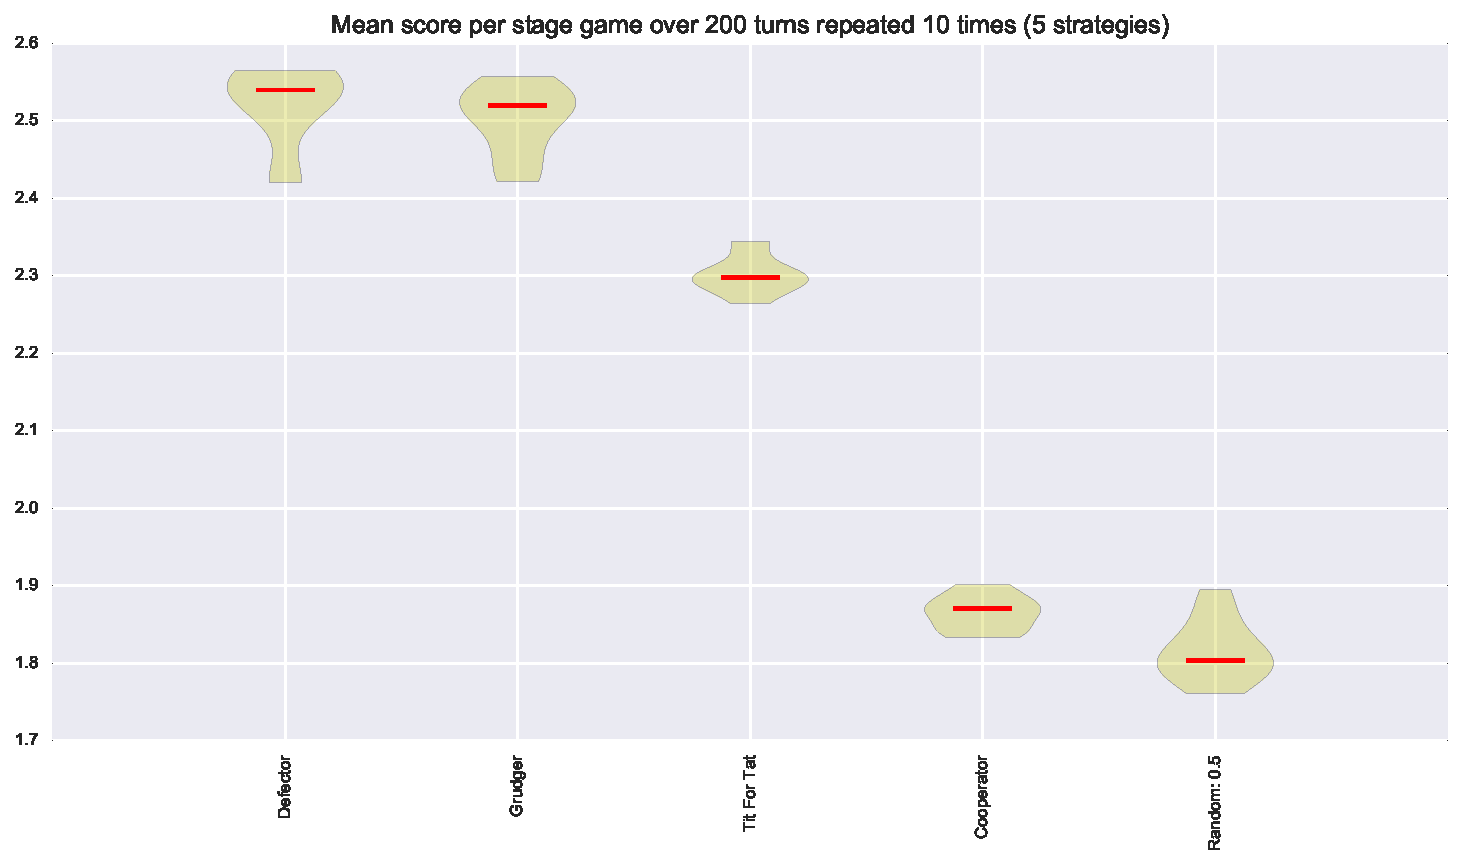
\includegraphics[width=.75\textwidth]{../img/demo_tournament.pdf}
		\caption{The results from a simple tournament.}
		\label{fig:demo_tournament}
	\end{subfigure}
	\begin{subfigure}{.5\textwidth}
		\centering
		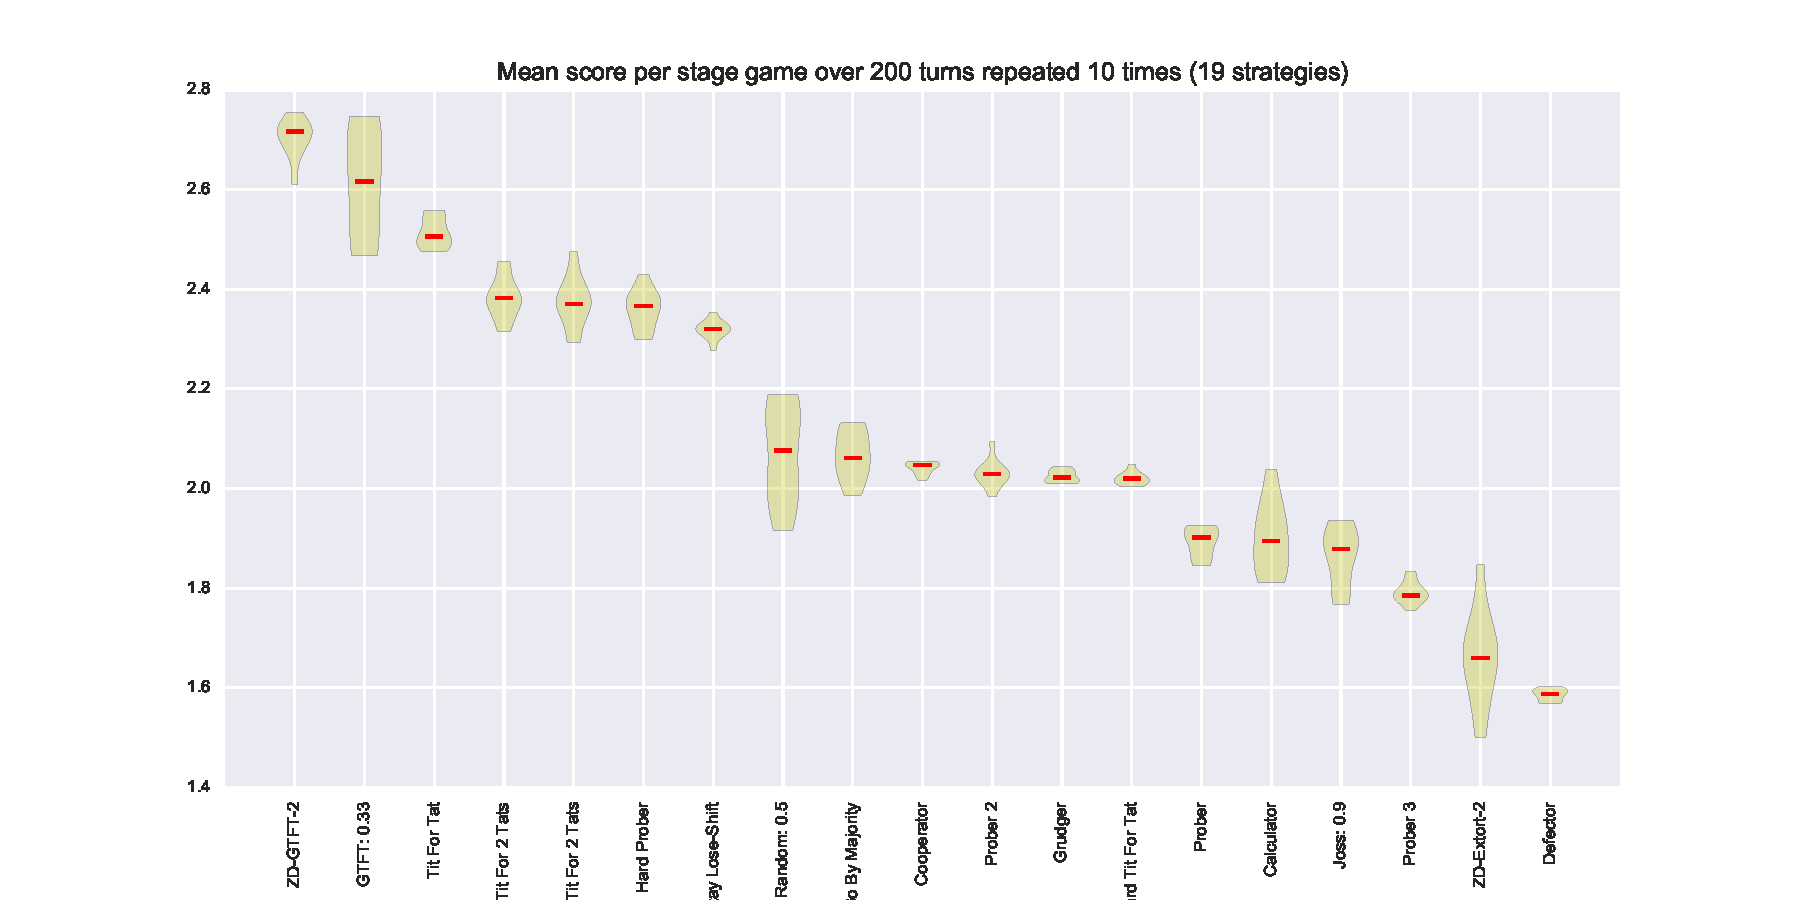
\includegraphics[width=.75\textwidth]{../img/stewart_tournament.pdf}
		\caption{The results from \cite{Stewart2012}.}
		\label{fig:stewart_tournament}
	\end{subfigure}
	\caption{Summary plots produced by the library.}
\end{figure}

Figure~\ref{fig:demo_tournament_commands} shows the very basic utilisation
of the library and further details can be found at the online documentation:
\url{http://axelrod.readthedocs.org}.

As stated in the \textbf{Introduction}, one of the main goals of the library
is to allow for the easy contribution of strategies. Doing this requires the
writing of a simple Python class (which can inherit from other predefined
classes). Full contribution guidelines can be found in the documentation.
As an example, Figures~\ref{fig:grudger} and~\ref{fig:grudger_test} show the source code for
the Grudger strategy as well as its corresponding test.

\begin{figure}[!hbtp]
    \begin{minted}[linenos, frame=lines]{python}
class Grudger(Player):
    """A player starts by cooperating however will defect if
       at any point the opponent has defected."""

    name = 'Grudger'
    classifier = {
        'memory_depth': float('inf'),  # Long memory
        'stochastic': False,
        'inspects_source': False,
        'manipulates_source': False,
        'manipulates_state': False
    }

    def strategy(self, opponent):
        """Begins by playing C, then plays D for the remaining
           rounds if the opponent ever plays D."""
        if opponent.defections:
            return D
        return C
    \end{minted}
    \caption{Source code for the Grudger strategy.}
    \label{fig:grudger}
\end{figure}



\begin{figure}[!hbtp]
    \begin{minted}[linenos, frame=lines]{python}
class TestGrudger(TestPlayer):

    name = "Grudger"
    player = axelrod.Grudger
    expected_classifier = {
        'memory_depth': float('inf'),  # Long memory
        'stochastic': False,
        'inspects_source': False,
        'manipulates_source': False,
        'manipulates_state': False
    }

    def test_initial_strategy(self):
        """
        Starts by cooperating
        """
        self.first_play_test(C)

    def test_strategy(self):
        """
        If opponent defects at any point then the player will defect forever
        """
        self.responses_test([C, D, D, D], [C, C, C, C], [C])
        self.responses_test([C, C, D, D, D], [C, D, C, C, C], [D])
    \end{minted}
    \caption{Test code for the Grudger strategy.}
    \label{fig:grudger_test}
\end{figure}

To date the library has had contributions from 24 contributors from a variety
of backgrounds. These contributions have been in terms of strategies. One
strategy is the creation of an undergraduate mathematics student with little
prior knowledge of programming. Multiple other strategies were written by a 15
year old secondary school student. Both of these students are authors of this
paper. As well as these strategy contributions, vital architectural
improvements to the library itself have also been received. You can see an
overview of the structure of the source code in Figure~\ref{fig:overview}.

\begin{figure}[!hbtp]
	\begin{subfigure}{.5\textwidth}
		\centering
		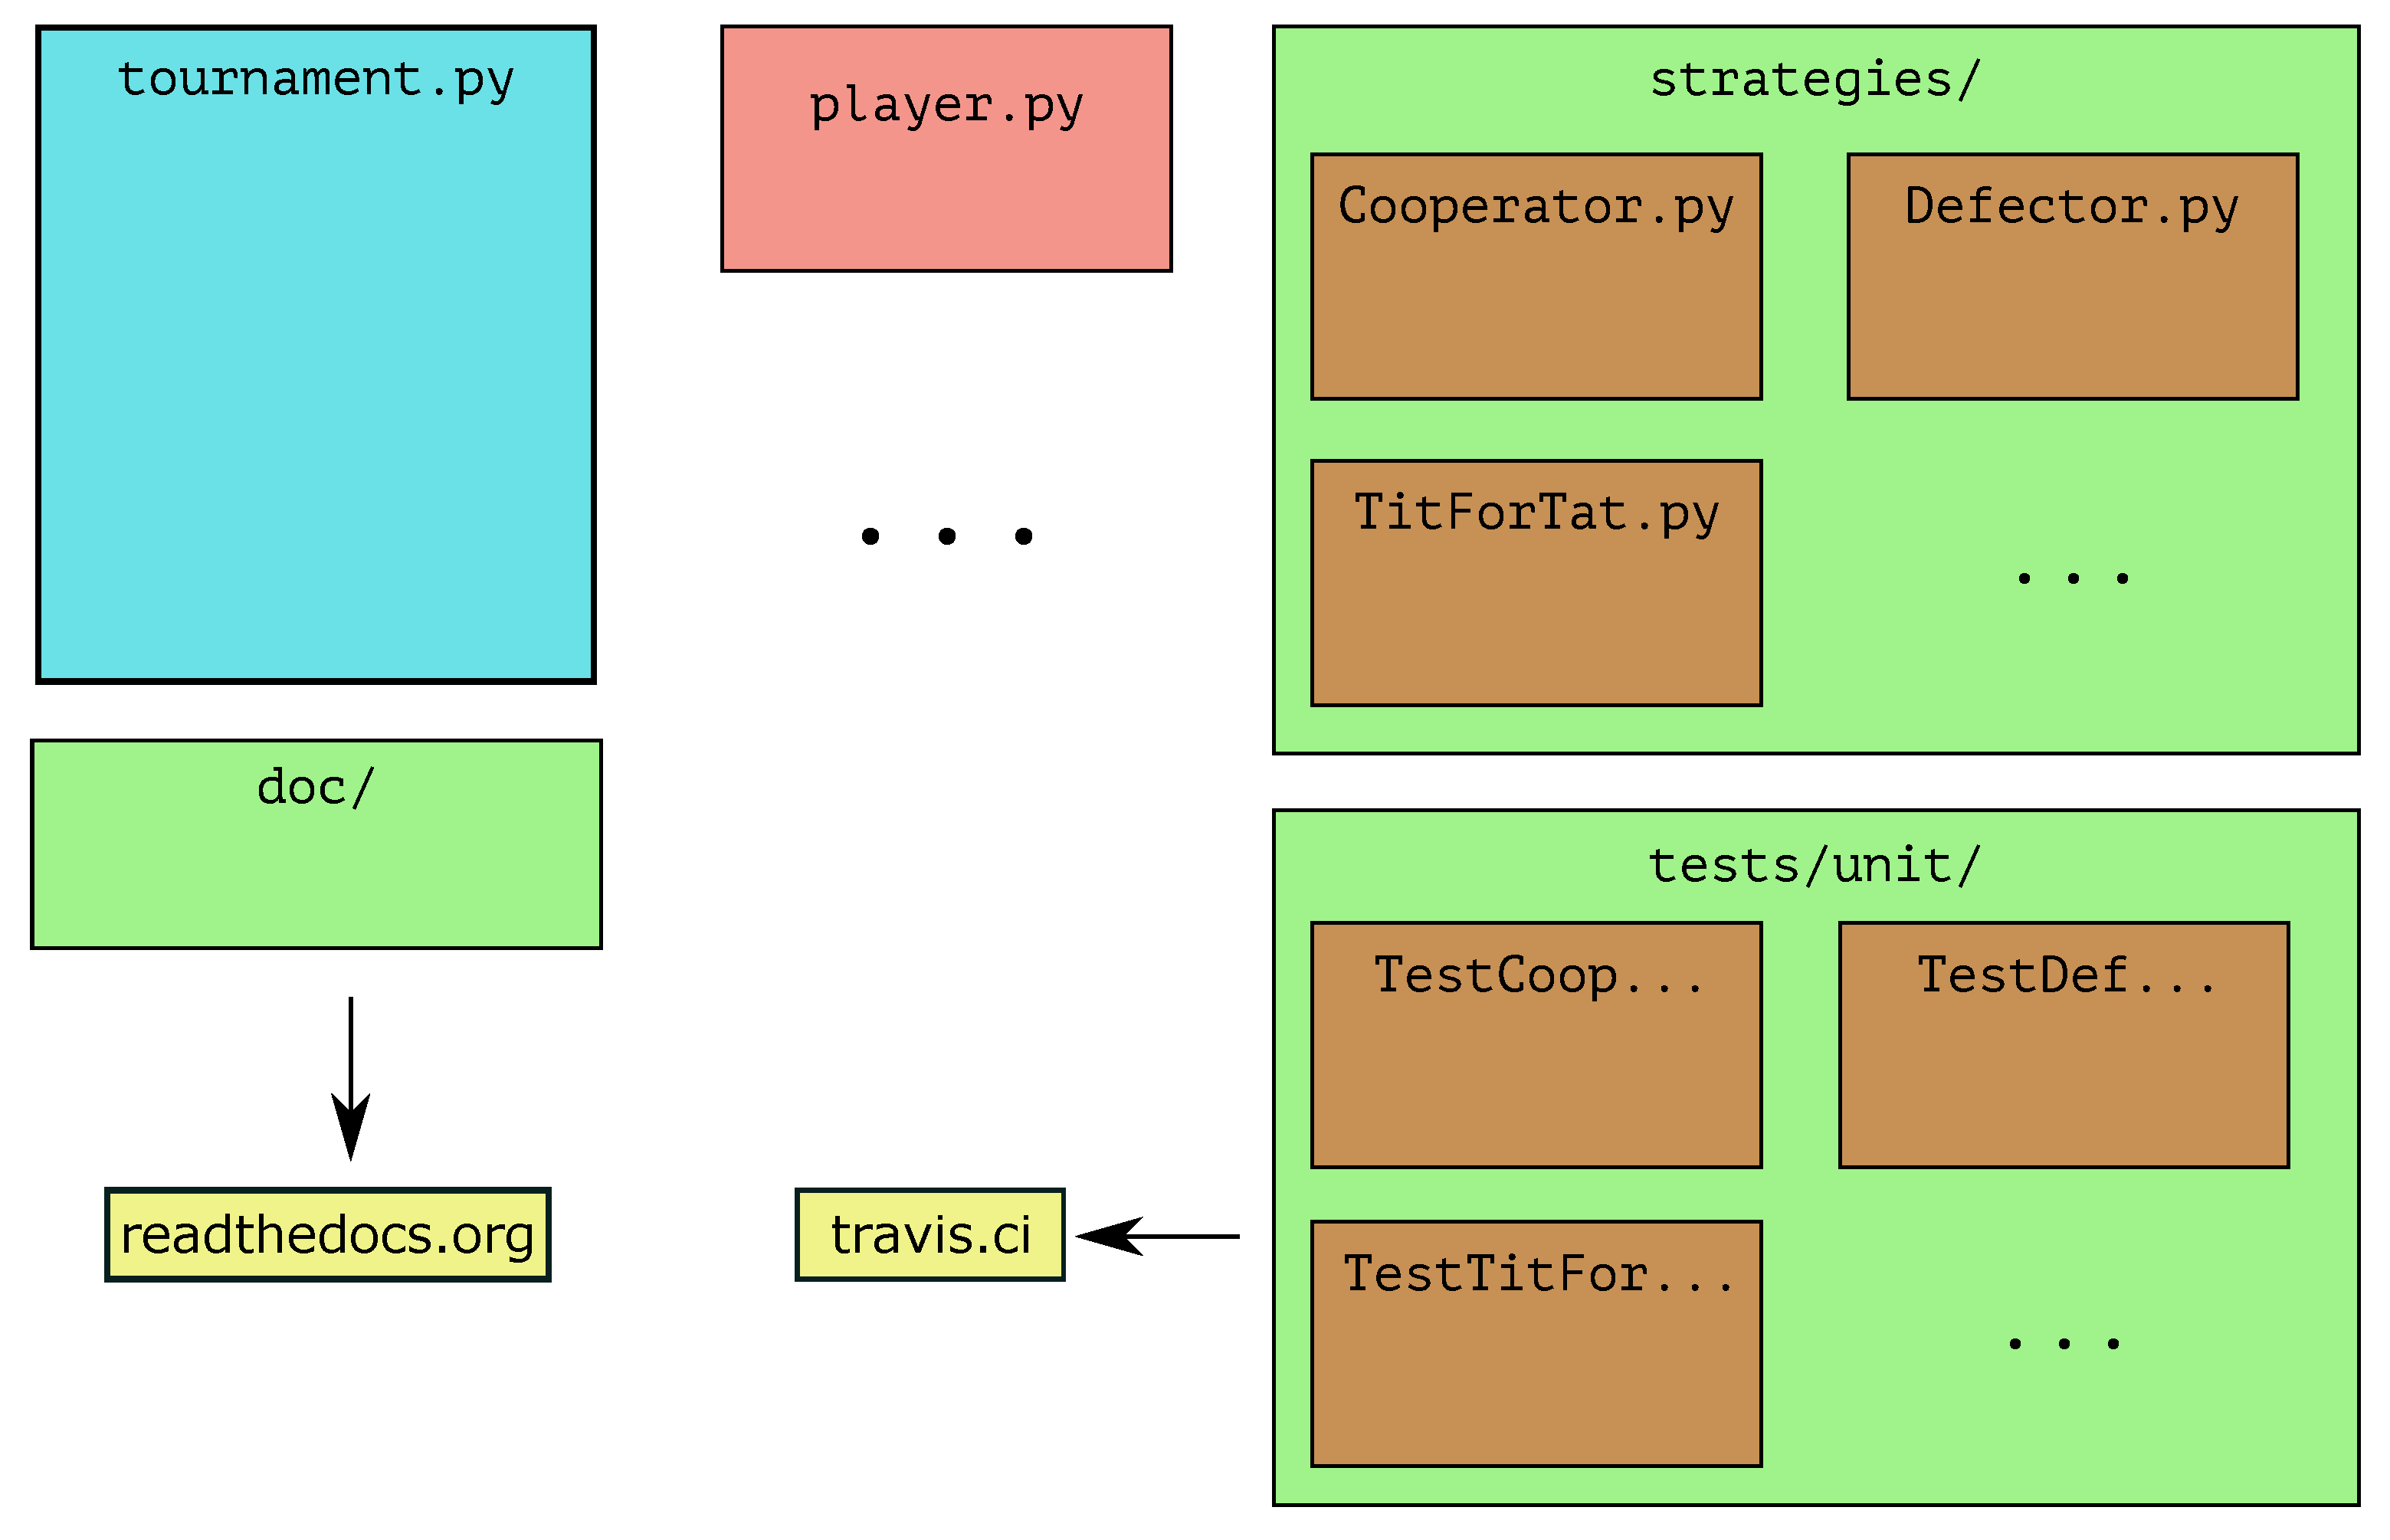
\includegraphics[width=.75\textwidth]{../img/outline_of_library.pdf}
		\caption{An overview of the source code.}
		\label{fig:overview}
	\end{subfigure}
	\begin{subfigure}{.5\textwidth}
		\centering
		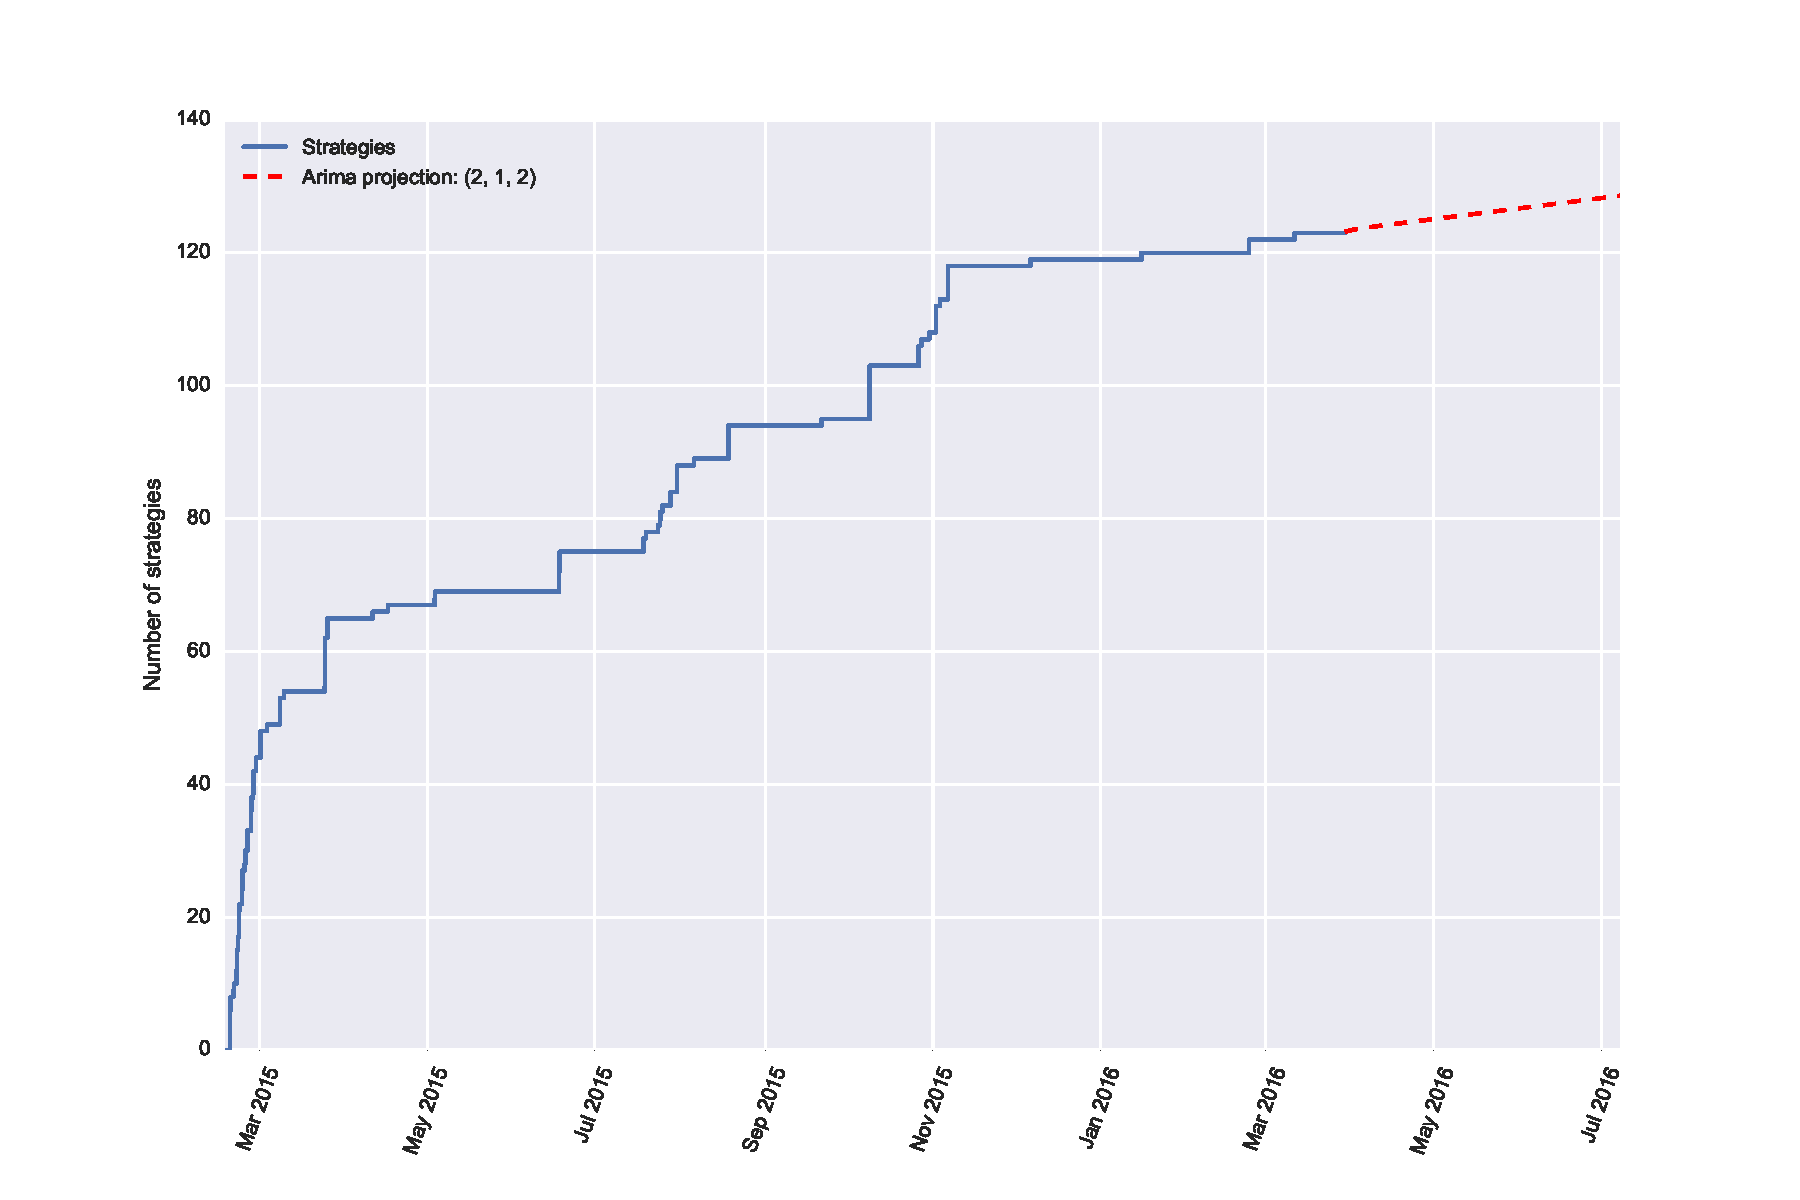
\includegraphics[width=.9\textwidth]{../img/number_of_strategies_with_arima_projection.pdf}
		\caption{The number of strategies included in the library}
		\label{fig:number_of_strategies_against_date}
	\end{subfigure}
	\caption{An overview of the library.}
\end{figure}

\section*{New strategies, tournaments and implications}\label{sec:new-strategies-and-implications}

Due to the open nature of the library the number of strategies included has
grown at a fast pace, as can be seen in
Figure~\ref{fig:number_of_strategies_against_date}. Despite this, due to
previous research being done in an irreproducible manner with, for example, no
source code and/or vaguely described strategies, not all previous tournaments
can yet be reproduced. In fact, some of the early tournaments might be
impossible to reproduce as the source code is forever lost. This library aims
to prevent this from happening again in the future.

One tournament that is possible to reproduce is that of
\cite{Stewart2012}. The strategies used in that tournament are the following:

\begin{multicols}{2}
    \begin{enumerate}[noitemsep,topsep=0pt]
        \item Cooperator
        \item Defector
        \item ZD-Extort-2
        \item Joss: 0.9
        \item Hard Tit For Tat
        \item Hard Tit For 2 Tats
        \item Tit For Tat
        \item Grudger
        \item Tit For 2 Tats
        \item Win-Stay Lose-Shift
        \item Random: 0.5
        \item ZD-GTFT-2
        \item GTFT: 0.33
        \item Hard Prober
        \item Prober
        \item Prober 2
        \item Prober 3
        \item Calculator
        \item Hard Go By Majority
    \end{enumerate}
\end{multicols}

This can be reproduced as shown in Figure~\ref{fig:stewart-code}, which gives
the plot of Figure~\ref{fig:stewart_tournament}.

\begin{figure}[!hbtp]
    \begin{minted}[linenos, frame=lines]{python}
>>> import axelrod

>>> strategies = [axelrod.Cooperator(),
...               axelrod.Defector(),
...               axelrod.ZDExtort2(),
...               axelrod.Joss(),
...               axelrod.HardTitForTat(),
...               axelrod.HardTitFor2Tats(),
...               axelrod.TitForTat(),
...               axelrod.Grudger(),
...               axelrod.TitFor2Tats(),
...               axelrod.WinStayLoseShift(),
...               axelrod.Random(),
...               axelrod.ZDGTFT2(),
...               axelrod.GTFT(),
...               axelrod.HardProber(),
...               axelrod.Prober(),
...               axelrod.Prober2(),
...               axelrod.Prober3(),
...               axelrod.Calculator(),
...               axelrod.HardGoByMajority()]
>>> tournament = axelrod.Tournament(strategies)
>>> results = tournament.play()
>>> plot = axelrod.Plot(results)
>>> plot.boxplot()
    \end{minted}
    \caption{Source code for reproducing the tournament of \cite{Stewart2012}}
    \label{fig:stewart-code}
\end{figure}

In parallel to the Python library, a tournament is being kept up to date that
pits all available strategies against each other. Figure~\ref{fig:tournament}
shows the results from the full tournament which can also be seen (in full
detail) here: \url{http://axelrod-tournament.readthedocs.org/}.

\begin{figure}[!hbtp]
	\centering
	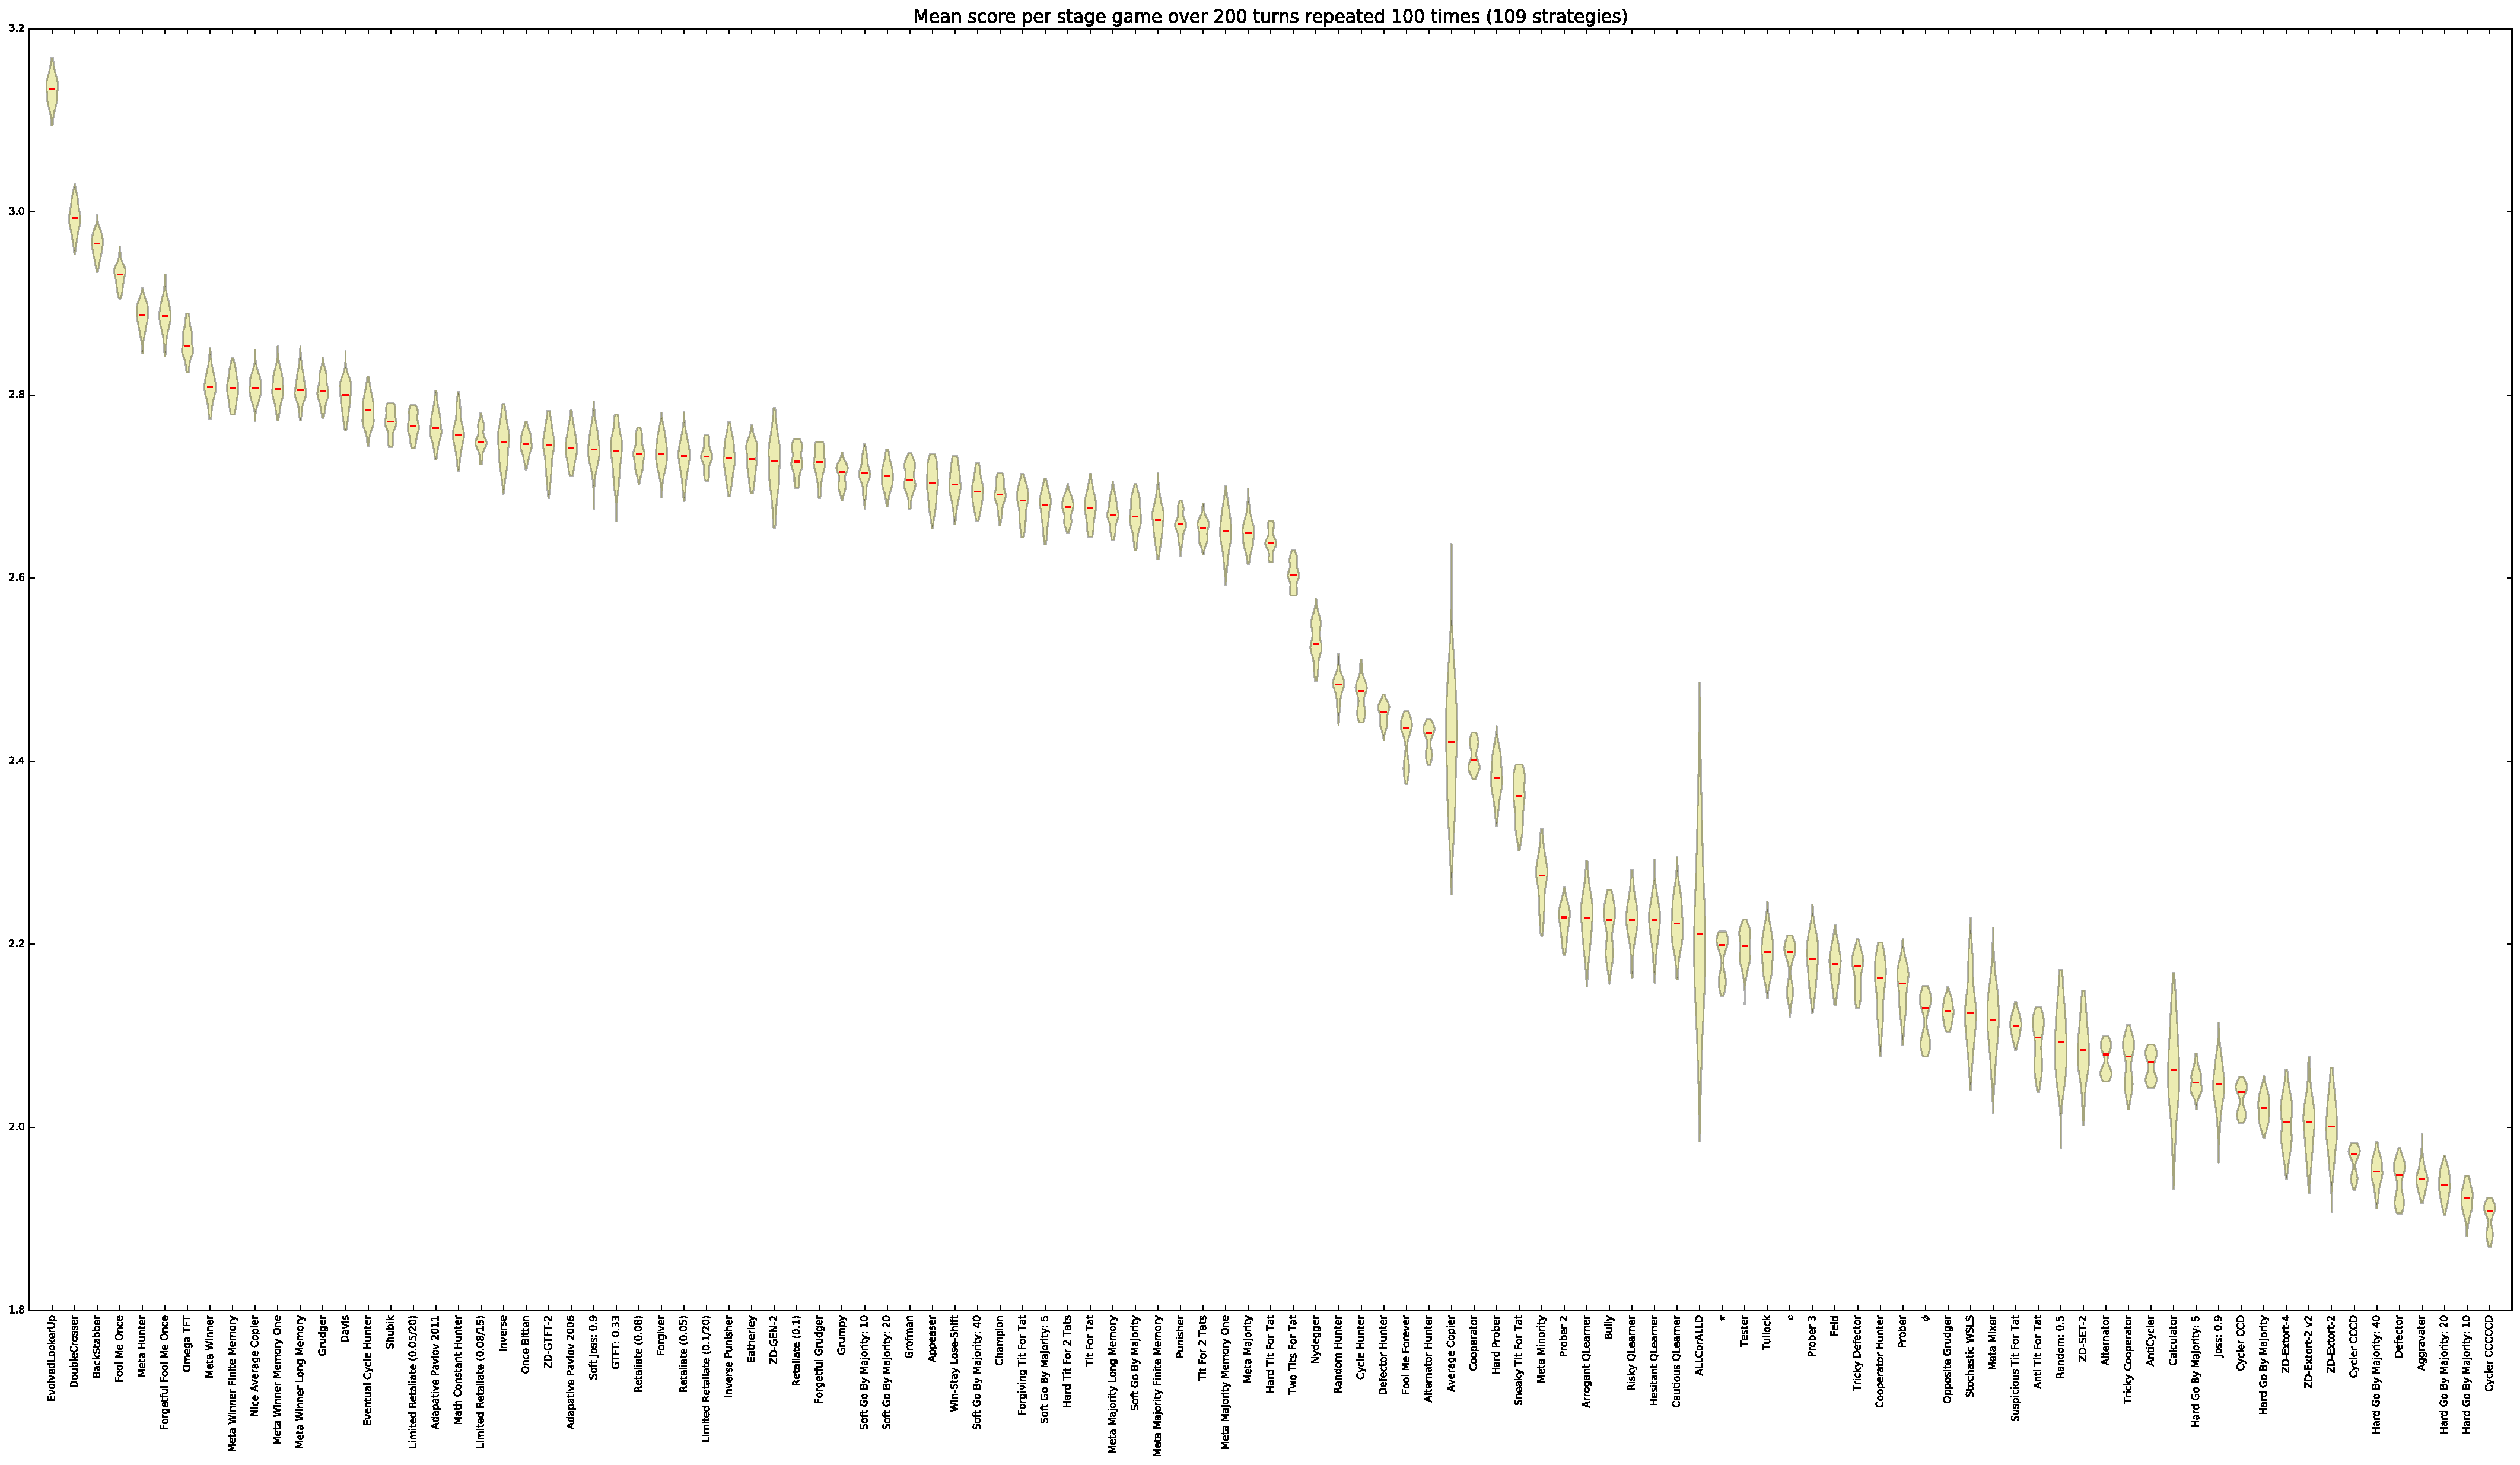
\includegraphics[width=.75\textwidth]{../img/tournament.pdf}
	\caption{Results from the library tournament (2016-03-31)}
	\label{fig:tournament}
\end{figure}

The current winning strategy is a novel strategy called: Looker Up. This is a
strategy that maps a given set of states to actions. The state space is defined
generically by \(m, n\) so as to map states to actions as shown
in~(\ref{equ:example_of_lookerup}).

\begin{equation}
	(\underbrace{(C, D, D, D, C, D, D, C)}_{m\text{ first actions by opponent}},
	\overbrace{((C, C), (C, C))}^{n\text{ last pairs of actions}}) \to D
	\label{equ:example_of_lookerup}
\end{equation}

The example of (\ref{equ:example_of_lookerup}) is an incomplete illustration of
the mapping for \(m=8, n=2\). Intuitively, this state space uses the initial
plays of the opponent to gain some information about its intentions whilst still
taking into account the recent play. The actual winning strategy is an instance
of the framework for \(m=n=2\) for which a particle swarm algorithm has been
used to train it, the second placed strategy was trained with an evolutionary
algorithms. More details of this can be found in \cite{Jones2015, George2016}.
In \cite{Knight2015} experiments are described that evaluate how the second
placed strategy behaves in environments other than those in which it was trained
and it continues to perform strongly.

There are various other insights that have been gained from ongoing open
research on the library. These include:

\begin{itemize}[noitemsep,topsep=0pt]
    \item A closer look at zero determinant strategies, showing that
        extortionate strategies obtain a large number of wins \textit{but} do
        not perform particularly well. This is relevant given the findings of
        \cite{Stewart2012} in which zero determinant strategies are shown to be
        able to perform better than any other strategy. This finding extends
        to noisy tournaments (which are also implemented in the library).
    \item This negative relationship between wins and performance does not
        generalise. There are some strategies that perform well, both in terms
        of matches won and overall performance: Back stabber, Double crosser,
        Looker Up, and Fool Me Once. These strategies continue to perform well in noisy
        tournaments, however some of these have knowledge of the length of the
        game (Back stabber and Double crosser). This is not necessary to rank
        well in both wins and score as demonstrated by Looker Up and Fool Me
        Once.
    \item Strategies like Looker Up and Meta Hunter seem to be generally
        cooperative yet still exploit naive strategies. The MetaHunter strategy
        is a particular type of Meta strategy which uses a variety of other
        strategy behaviours to choose a best action. These strategies perform
        very well in general and continue to do so in noisy tournaments.
\end{itemize}

Details for the above can be found in \cite{Harper2015}.

\section*{(2) Availability}\label{sec:availability}

\section*{Operating system}

The Axelrod library runs on all major operating systems: Linux, Mac OSX and
Windows.

\section*{Programming language}

The library is continuously tested for Python 2.7, 3.3, 3.4 and 3.5.

\section*{Additional system requirements}

There are no specific additional system requirements.

\section*{Support}

Support is readily available in multiple forms:

\begin{itemize}[noitemsep,topsep=0pt]
    \item An online chat channel:
        \url{https://gitter.im/Axelrod-Python/Axelrod}.
    \item An  email group:
        \url{https://groups.google.com/forum/#!topic/axelrod-python}.
\end{itemize}

\section*{Dependencies}

The following Python libraries are required dependencies:

\begin{multicols}{3}
    \begin{itemize}[noitemsep,topsep=0pt]
        \item Numpy 1.9.2:
        \item Matplotlib 1.4.2:
        \item Cloudpickle  0.1.1:
        \item Hypothesis  3.0:
        \item Testfixtures  4.9.1:
    \end{itemize}
\end{multicols}

\section*{List of contributors}

The names of all the contributors are not known: as these were mainly done
through Github and certain have not provided their name or responded to a
request for further details. Here is an incomplete list:

\begin{multicols}{2}
    \begin{itemize}[noitemsep,topsep=0pt]
        \item {Owen Campbell}
        \item {Mark Harper}
        \item {Vincent Knight}
        \item {Karol Langner}
        \item {James Campbell}
        \item {Thomas Campbell}
        \item {Alex Carney}
        \item {Martin Chorley}
        \item {Cameron Davidson-Pilon}
        \item {Kristian Glass}
        \item {Tom{\'a}{\v s} Ehrlich}
        \item {Martin Jones}
        \item {Georgios Koutsovoulos}
        \item {Marissa Tibble}
        \item {Jochen M{\"u}ller}
        \item {Geraint Palmer}
        \item {Paul Slavin}
        \item {Timothy Standen}
        \item {Luis Visintini}
        \item {Karl Molden}
        \item {Jason Young}
        \item {Andy Boot}
        \item {Anna Barriscale}
    \end{itemize}
\end{multicols}

\section*{Software location:}

{\bf Archive}

\begin{description}[noitemsep,topsep=0pt]
    \item[Name:] Zenodo
    \item[Persistent identifier:]
\href{https://zenodo.org/record/45187}{10.5281/zenodo.45187}
    \item[Licence:] MIT
    \item[Publisher:]  Vincent Knight
    \item[Version published:] Axelrod: Alternator Release. v0.0.28
    \item[Date published:] 2016-01-26
\end{description}

{\bf Code repository}

\begin{description}[noitemsep,topsep=0pt]
    \item[Name:] Github
    \item[Identifier:] \url{https://github.com/Axelrod-Python/Axelrod}
    \item[Licence:] MIT
    \item[Date published:] 2015-02-16
\end{description}

\section*{Reuse potential}\label{sec:reuse}

The Axelrod library has been designed with sustainable software practice in
mind. There is an extensive documentation suite:
\url{axelrod.readthedocs.org/en/latest/}. Furthermore, there is a growing set
of example Jupyter notebooks available here:
\url{https://github.com/Axelrod-Python/Axelrod-notebooks}.

The ability to have readily available a large number of strategies makes this
tool an excellent and obvious example of the benefits of open research which
should positively impact the game theoretic community.
This has been evidenced by the work described: the library has already shown
it's potential for reuse.

\section*{Conclusion}

This paper has presented a game theoretic software package that aims to address
reproducibility of research into the Iterated Prisoner's Dilemma. The open
nature of the development of the library has lead rapidly to the inclusion of
many well known strategies, many novel strategies, and new and recapitulated
insights.

The capabilities of the library mentioned above are not at all comprehensive, a
list of the current abilities include:

\begin{itemize}[noitemsep,topsep=0pt]
    \item Noisy tournaments;
    \item Tournaments with probabilistic ending of interactions;
    \item Ecological analysis of tournaments;
    \item Morality metrics based on \cite{Singer-Clark2014};
    \item Transformation of strategies (in effect giving an infinite number of
        strategies);
    \item Classification of strategies according to multiple dimensions.
    \item Gathering of full interaction history for all interactions.
\end{itemize}

These capabilities are constantly being updated.

\section*{Acknowledgements}

The authors would like to thank all contributors. Also, they thank
Robert Axelrod himself for his well wishes with the library.

\section*{Competing interests}

The authors declare that they have no competing interests.

\printbibliography
\end{document}
